\documentclass{report}
\usepackage{graphicx}
\usepackage{hyperref}
\usepackage[left=2cm,right=2cm,top=2cm,bottom=1.5cm]{geometry}
\usepackage{booktabs}
\usepackage{array}
\usepackage{caption}
\usepackage[list=true,listformat=simple]{subcaption}
\usepackage{multirow}
\usepackage{setspace}
\usepackage{titlesec}
\usepackage{pifont}
\usepackage{lscape}
\usepackage{url}
\usepackage{hyperref}
\usepackage{comment}
\usepackage{array}
\usepackage{float}
\newcolumntype{P}[1]{>{\centering\arraybackslash}p{#1}}

\usepackage{listings}
\usepackage{color}
\usepackage{pythonhighlight}

\setcounter{secnumdepth}{4}
\makeatletter
\setlength\@fptop{0pt}             % default: '0\p@ \@plus 1fil'
\setlength\@fpsep{2\baselineskip}  % default: '8\p@ \@plus 2fil'
\makeatother


% Title Page
\title{PSSE Contingency Analysis - Year 0 Topology 0 }
\author{Jessla Varaparambil Abdul Kadher}
\begin{document}
\maketitle


\tableofcontents
\listoffigures
\listoftables

\newpage

\chapter{Introduction}

\section{Study Description}

The Year 0 Topology 0 contingency analysis of the hypothetical SAVNW system is carried out to report the branches reporting loading greater than 100\% and buses reporting upper and lower voltage limit violations. 

\begin{figure}[h!]
   \centering 
   \includegraphics[scale=0.5]{y0t0}
   \caption{Single Line Diagram Year 0, Topology 0} 
   \label{fig:y0t0}
\end{figure}

For the hypothetical SAVNW system, the Year 0 Topology 0 of the system represents the present year system as shown in Figure ~\ref{fig:y0t0}. There are 6 generators in 3 areas. Total installed capacity of the system is the sum of firm capacity provided by 6 generating units and equals 4153.25 MW. 

Detailed analysis of Year 0 Topology 0 base case was carried out and can be found \href{https://htmlpreview.github.io/?https://github.com/jessla89/PSSE-Data-Extraction/blob/main/Analysis_Topology_0.html}{here}. The combined total generation in all areas of 2765 MW is serving a total load of 2723 MW with the generators 102 – NUC-B, 211-HYDRO\_G, 3018-CATDOG\_G operating at their nominal power output of 700 MW, 500 MW and 90 MW respectively. The swing generator in each area operates to meet the load, loss and interchange criteria. The desired interchange for all the scenarios studied is highlighted in Figure ~\ref{fig:year0totals}. For all the scenarios studied the desired interchange from FLAPCO to LIGHTCO is 100 MW, and from FLAPCO to WORLD is 150 MW. 

\begin{figure}[h!]
   \centering 
   \includegraphics[scale=0.6]{year_0_totals}
   \caption{System Totals for Year - 0, Topology - 0} 
   \label{fig:year0totals}
\end{figure}


\chapter{Contingency Analysis}


AC contingency calculation was conducted on the hypothetical SAVNW system for Year 0 Topology 0. The configuration files used are:
\begin{itemize}
\item Subsystem file savnw.sub - Studied subsystems of the studied case defined via the Subsystem Definition data file (Figure ~\ref{fig:sub})
\item Monitor file savnw.mon - Monitored Element Data File identifies the branches that are to be monitored for flow violations and the buses that are to be monitored for voltage violations (Figure ~\ref{fig:mon})
\item  Contingency file savnw.con - Contingency cases that are to be tested are defined in the Contingency Definition data file (Figure ~\ref{fig:con})
\end{itemize}

\begin{figure}[H]
   \centering 
   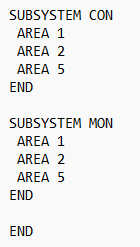
\includegraphics[scale=0.6]{sub.png}
   \caption{The subsystem file corresponding to Year 1 Topology 1} 
   \label{fig:sub}
\end{figure}

\begin{figure}[H]
   \centering 
   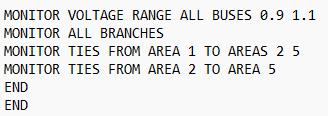
\includegraphics[scale=0.6]{mon.png}
   \caption{The monitored file corresponding to Year 1 Topology 1} 
   \label{fig:mon}
\end{figure}

\begin{figure}[H]
   \centering 
   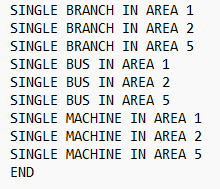
\includegraphics[scale=0.6]{con.png}
   \caption{The contingency file corresponding to Year 1 Topology 1} 
   \label{fig:con}
\end{figure}


The API DFAX\_2 is used to construct distribution factor data files corresponding to the case .sav file, and the defined .sub, .mon, .con configuration files.
By running the AC contingency calculation function ACCC\_WITH\_DSP\_3, the contingency solution output .acc files is obtained.

Python code to conduct AC contingency calculation is:

\begin{python}
import psspy
psspy.case(r"""savnw.sav""")
psspy.fdns([0,1,0,0,0,0,99,0])
psspy.dfax_2([1,1,0],r"""savnw.sub""",r"""savnw.mon""",r"""savnw.con""",r"""savnw.dfx""")
psspy.accc_with_dsp_3(0.1,[0,0,0,0,1,2,0,0,0,2,0],r"""CON""",r"""savnw.dfx""",r"""savnw.acc""","","","")
\end{python}

Using the contingency solution output file savnw.acc, the results is exported as an excel file for further analysis. The results exported are ACCC Analysis Summary, Monitored Branch Flow (MVA), Monitored Bus Voltage.

Python code to export AC contingency solution output file as excel is: 

\begin{python}
import psspy
import pssexcel
pssexcel.accc('savnw.acc', ['s','b'], colabel='',stype='contingency', busmsm=0.5, sysmsm=5.0,
                rating='a', namesplit=False,xlsfile='out.xlsx', sheet='', overwritesheet=True, show=False, ratecon='b',
                baseflowvio=False,basevoltvio=False, flowlimit=100.0, flowchange=0.0, voltchange=0.0,swdrating='a',
                swdratecon='b',baseswdflowvio=False,basenodevoltvio=False,overloadreport=False)
\end{python}

Contingency analysis was carried out in PSSE for the studied case for Year 0 Topology 0. It was seen that the power flow solution did not converge for some of the tested contingencies. For the studied case, 42 contingencies were converged out of the 47 contingencies tested, the contingencies not converged are UNIT 206(1), SING OPN LIN   14 205-206(1), BUS 152, BUS 154, and BUS 201.

For the converged contingencies for the studied case, the result of the contingency analysis is analysed to check for branch overload ($ > 100\%$) and out of range bus voltage violations (lower emergency limit $ < 0.9 PU $ and upper emergency limit $ > 1.1 PU$). It was seen that for some of the contingencies there were no branch overload or bus voltage violations reported. Rest of the contingencies violating branch overload and bus voltage emergency range violation are reported. Chapter ~\ref{violations} gives the observed branch flow violations, upper and lower emergency voltage violations for the studied case and the Chapter ~\ref{conclusion} summarises the results of all the analysis carried out on Year 0, Topology 0 of the hypothetical SAVNW system. 


\chapter{Contingency Limit Violations}
\label{violations}
\section{Introduction}
In this chapter, for Year 0, Topology 0, the branches that are loaded more than 100\% of their rating, and buses violating the upper and lower emergency ratings are reported. 

\section{Branch Overload Violation}
For Year 0, Topology 0, out of the 34 branches in the system, 8 branches reporting a loading greater than 100\% are given in Table ~\ref{year0loading}. 

\begin{table}[H]
\caption{Loading Violations Year 0 Topology 0}
\label{year0loading}
\centering
\scalebox{0.9}{\begin{tabular}{llrrrr}
\toprule
Branch & Contingency & MVA Flow & AMP Flow & Rate & Loading \\
\midrule
3001-3003(1) & SING OPN LIN   1 101-151(1) & 532.205 & 515.011 & 300.000 & 171.670 \\
153-154(1) & SING OPN LIN   11 202-203(1) & -349.967 & 359.164 & 350.000 & 102.618 \\
3001-3003(1) & BUS 151 & 1050.651 & 1057.534 & 300.000 & 352.511 \\
3001-3011(1) & BUS 151 & -1648.816 & 1648.816 & 1560.000 & 105.693 \\
3003-3005(1) & BUS 151 & 517.274 & 528.764 & 350.000 & 151.075 \\
3003-3005(2) & BUS 151 & 517.274 & 528.764 & 350.000 & 151.075 \\
3005-3007(1) & BUS 151 & -353.065 & 378.495 & 350.000 & 108.141 \\
153-154(1) & BUS 203 & -348.675 & 357.543 & 350.000 & 102.155 \\
153-154(1) & BUS 205 & -310.402 & 352.007 & 350.000 & 100.573 \\
154-203(1) & BUS 205 & 289.401 & 328.191 & 250.000 & 131.277 \\
3001-3003(1) & UNIT 101(1) & 532.205 & 515.011 & 300.000 & 171.670 \\
\bottomrule
\end{tabular}}
\end{table}

For Year 0, Topology 0 the branches reporting a loading greater than 130\% are the branches 3001-3003(1), 3003-3005(1), 3003-3005(2), 154-203(1). The branch 3001-3003(1) reported the violation for single line open contingency SING OPN LIN   1 101-151(1), for bus fault BUS 151, and for unit fault UNIT 101(1). The branches 3003-3005(1) and 3003-3005(2) reported the branch loading violation for the bus fault BUS 151, and the branch 154-203(1) reported a violation for the bus fault BUS 205. Further analysis would be required to assess the steady state and transient stability of the system to these faults as the loading violation is quite high for all these contingencies with the bus fault BUS 151 reporting a loading of as high as 353.5\%.  


\section{Upper Emergency Bus Voltage Violation}

For Year 0, Topology 0, there were no buses reporting an upper emergency voltage violation of greater than 1.1 PU. 


\section{Lower Emergency Bus Voltage Violation}

For Year 0, Topology 0, the only bus reporting lower emergency voltage violation is the bus 154 for a bus fault at bus 205 labelled BUS 205 as can be seen from Table ~\ref{year0volt}.

\begin{table}[H]
\caption{Lower Emergency Voltage Violations Year 0 Topology 0}
\label{year0volt}
\centering
\scalebox{0.9}{
\begin{tabular}{llrrrr}
\toprule
Bus Number & Contingency & Base Voltage & Contingency Voltage & Deviation & Range Violation \\
\midrule
154 & BUS 205 & 0.976 & 0.882 & -0.094 & -0.018 \\
\bottomrule
\end{tabular}}
\end{table}

\chapter{Conculsion}
\label{conclusion} 

The contingency analysis was carried out on the hypothetical SAVNW study system for the Year 0, Topology 0 to study the bus fault, single line open fault, unit fault contingencies. Out of all the studied contingencies, the contingencies for which the system did not converge are the contingencies UNIT 206(1), SING OPN LIN   14 205-206(1), BUS 152, BUS 154, and BUS 201.

For the converged contingency scenarios, Chapter \ref{violations} reported the branch overload, upper and lower limit voltage violations. From the branch overload table, Table \ref{year0loading} branches reporting loading greater than 130\% were the branches 3001-3003(1), 3003-3005(1), 3003-3005(2), and 154-203(1). There were no upper limit voltage violations reported for any of the studied buses. Lower limit voltage violations were reported by the bus 154 for a bus fault BUS 205 for Year 0 Topology 0 (Table ~\ref{year0volt}). 

The branch reporting the greatest number of overloaded violations are the branches 3001-3003(1) and 153-154(1) with 3 violations each as can be seen from Table ~\ref{count_bran_overload}. The contingency causing the most number of branch overload violation is the bus fault contingency BUS 151 with 5 overload violation followed by the bus fault contingency BUS 205 with 2 violations as can be seen from Table ~\ref{count_cont_overload}. 

\chapter*{Appendix}
\addcontentsline{toc}{chapter}{Appendix}
\label{chapter:app}



\begin{table}[H]
\caption{Overload Count - Branch}
\label{count_bran_overload}
\centering
\scalebox{0.8}{\begin{tabular}{lr}
\toprule
Branch & Overload Counts \\
\midrule
3001-3003(1) & 3 \\
153-154(1) & 3 \\
3001-3011(1) & 1 \\
3003-3005(1) & 1 \\
3003-3005(2) & 1 \\
3005-3007(1) & 1 \\
154-203(1) & 1 \\
\bottomrule
\end{tabular}}
\end{table}


\begin{table}[H]
\caption{Overload Count - Contingency}
\label{count_cont_overload}
\centering
\scalebox{0.8}{\begin{tabular}{lr}
\toprule
Contingency & Overload Counts \\
\midrule
BUS 151 & 5 \\
BUS 205 & 2 \\
SING OPN LIN   1 101-151(1) & 1 \\
SING OPN LIN   11 202-203(1) & 1 \\
BUS 203 & 1 \\
UNIT 101(1) & 1 \\
\bottomrule
\end{tabular}}
\end{table}



\end{document}